\documentclass{beamer}
\usepackage{amsmath}
\usepackage[english]{babel} %set language; note: after changing this, you need to delete all auxiliary files to recompile
\usepackage[utf8]{inputenc} %define file encoding; latin1 is the other often used option
\usepackage{csquotes} % provides context sensitive quotation facilities
\usepackage{graphicx} %allows for inserting figures
\usepackage{booktabs} % for table formatting without vertical lines
\usepackage{textcomp} % allow for example using the Euro sign with \texteuro
\usepackage{stackengine}
\usepackage{wasysym}
\usepackage{tikzsymbols}
\usepackage{textcomp}
\usepackage{adjustbox}
\usepackage{xcolor}
\usepackage[table]{xcolor}
\usepackage[dvipsnames]{xcolor}
% ELIMINAR COMANDOS DE NAVEGACION%%%%%%%%%%%
\setbeamertemplate{navigation symbols}

%\newcommand{\bubblethis}[2]{
 %       \tikz[remember picture,baseline]{\node[anchor=base,inner sep=0,outer sep=0]%
 %       (#1) {\underline{#1}};\node[overlay,cloud callout,callout relative pointer={(0.2cm,-0.7cm)},%
 %       aspect=2.5,fill=yellow!90] at ($(#1.north)+(-0.5cm,1.6cm)$) {#2};}%
 %   }%
%\tikzset{face/.style={shape=circle,minimum size=4ex,shading=radial,outer sep=0pt,
 %       inner color=white!50!yellow,outer color= yellow!70!orange}}

%% Some commands to make the code easier
\newcommand{\emoticon}[1][]{%
  \node[face,#1] (emoticon) {};
  %% The eyes are fixed.
  \draw[fill=white] (-1ex,0ex) ..controls (-0.5ex,0.2ex)and(0.5ex,0.2ex)..
        (1ex,0.0ex) ..controls ( 1.5ex,1.5ex)and( 0.2ex,1.7ex)..
        (0ex,0.4ex) ..controls (-0.2ex,1.7ex)and(-1.5ex,1.5ex)..
        (-1ex,0ex)--cycle;}
\newcommand{\pupils}{
  %% standard pupils
  \fill[shift={(0.5ex,0.5ex)},rotate=80] 
       (0,0) ellipse (0.3ex and 0.15ex);
  \fill[shift={(-0.5ex,0.5ex)},rotate=100] 
       (0,0) ellipse (0.3ex and 0.15ex);}

\newcommand{\emoticonname}[1]{
  \node[below=1ex of emoticon,font=\footnotesize,
        minimum width=4cm]{#1};}
\usepackage{scalerel}
\usetikzlibrary{positioning}
\usepackage{xcolor,amssymb}
\newcommand\dangersignb[1][2ex]{%
  \scaleto{\stackengine{0.3pt}{\scalebox{1.1}[.9]{%
  \color{red}$\blacktriangle$}}{\tiny\bfseries !}{O}{c}{F}{F}{L}}{#1}%
}
\newcommand\dangersignw[1][2ex]{%
  \scaleto{\stackengine{0.3pt}{\scalebox{1.1}[.9]{%
  \color{red}$\blacktriangle$}}{\color{white}\tiny\bfseries !}{O}{c}{F}{F}{L}}{#1}%
}
\usepackage{fontawesome} % Social Icons
\usepackage{epstopdf} % allow embedding eps-figures
\usepackage{tikz} % allows drawing figures
\usepackage{amsmath,amssymb,amsthm} %advanced math facilities
\usepackage{lmodern} %uses font that support italic and bold at the same time
\usepackage{tikz}
\usepackage{tcolorbox}

\usefonttheme[onlymath]{serif} %set math font to serif ones

\definecolor{beamerblue}{rgb}{0.2,0.2,0.7} %define beamerblue color for later use
\definecolor{electricBlue}{RGB}{44,117,255}
%%% defines highlight command to set text blue
\newcommand{\highlight}[1]{{\color{blue}{#1}}}


%%%%%%% commands defining backup slides so that frame numbering is correct

\newcommand{\backupbegin}{
   \newcounter{framenumberappendix}
   \setcounter{framenumberappendix}{\value{framenumber}}
}
\newcommand{\backupend}{
   \addtocounter{framenumberappendix}{-\value{framenumber}}
   \addtocounter{framenumber}{\value{framenumberappendix}}
}

%%%% end of defining backup slides

%Specify figure caption, see also http://tex.stackexchange.com/questions/155738/caption-package-not-working-with-beamer
\setbeamertemplate{caption}{\insertcaption} %redefines caption to remove label "Figure".
%\setbeamerfont{caption}{size=\scriptsize,shape=\itshape,series=\bfseries} %sets figure  caption bold and italic and makes it smaller

\newtcolorbox{boxA}{
    fontupper = \bf,
    boxrule = 1.5pt,
    colframe = black % frame color
}
\newtcolorbox{boxB}{
    boxrule = 1.5pt,
    colframe = blue!70!black,, % frame color
    colback = blue!7!white,
}
\usetheme{Boadilla}

\usepackage{hyperref}


% --------------------
% Overall information
% --------------------
\title[Economía I]{Economía I \vspace{4mm}
\\ Magistral 7: El largo plazo y la oferta de la firma}
\date{}
\author[Riottini]{Franco Riottini}
\vspace{0.4cm}
\institute[]{Universidad de San Andrés} 

\begin{document}

\begin{frame}
\titlepage
\centering

\includegraphics[scale=0.2]{../Figures/logoUDESA.jpg} 
\end{frame}

\begin{frame}{Los costos de largo plazo}
\begin{itemize}
    \item En el largo plazo, la empresa puede ajustar cualquier cantidad de insumos requeridos para la producción. Es decir, \textbf{no hay insumos fijos} y, por ende, tampoco hay costos fijos. 
    \item Los costos de una empresa dependen de su escala y el tipo de tecnología de producción
    \item Empresas grandes pueden ser más rentables que las pequeñas debido diversas ventajas:
    \begin{itemize}
        \item Ventajas tecnológicas: producción a gran escala permite mejorar la especialización y bajar los costos.
        \item Ventajas de costos: por ejemplo, empresas grandes, con mayor poder de negociación, pueden comprar recursos en términos más favorable.
        \item Ventajas de demanda: por ejemplo, efectos de red (valor de la producción aumenta con el número de usuarios).
    \end{itemize}
\end{itemize}
\end{frame}

\begin{frame}{Costos Medios en el largo plazo}
    \centering
    \begin{tikzpicture}[scale=0.8, line cap=round, line join=round]
        \draw[->, thick] (0,0) -- (9,0) node[below] {\scriptsize Pizzas};
        \draw[->, thick] (0,0) -- (0,7) node[left] {\scriptsize CMe};
        \draw[thick, domain=0:3, smooth, variable=\x, color=electricBlue]
        plot (\x, {0.3*(\x-1.5)^2 + 3});
        \node at (1.5,4.1) {\scriptsize Haciendo};
        \node at (1.5,3.8) {\scriptsize pizzas en casa};
        \only<2->{
            \draw[thick, domain=2.7:5.9, smooth, variable=\x, color=electricBlue]
            plot (\x, {0.3*(\x-4.3)^2 + 2});
            \node at (4.3,3.2) {\scriptsize Haciendo pizzas};
            \node at (4.3,2.9) {\scriptsize en varios locales};
        }
        \only<3->{
            \draw[thick, domain=5.7:8.6, smooth, variable=\x, color=electricBlue]
            plot (\x, {0.3*(\x-7.1)^2 + 3});
            \node at (7.1,4.1) {\scriptsize El imperio};
            \node at (7.1,3.8) {\scriptsize de las pizzas};
        }
    \end{tikzpicture}
\end{frame}

\begin{frame}{Rendimientos a escala}
\begin{itemize}
    \item ¿Qué sucede con la producción cuando aumentamos la cantidad de insumos productivos en la misma proporción?
    \begin{itemize}
        \item La producción aumenta pero... ¿cuánto aumenta?
    \end{itemize}
    \item Si la producción aumenta más que proporcionalmente, entonces la función de producción exhibe rendimientos crecientes a escala (Economías de escala o costos decrecientes a escala)
    \item Si la producción aumenta proporcionalmente, entonces la función de producción exhibe rendimientos constantes a escala (Costos constantes a escala)
    \item Si la producción aumenta menos que proporcionalmente, entonces la función de producción exhibe rendimientos decrecientes a escala (Deseconomías de escala o costos crecientes a escala)
\end{itemize}
\end{frame}

\begin{frame}
    \frametitle{Costos en el largo plazo}
    \centering
    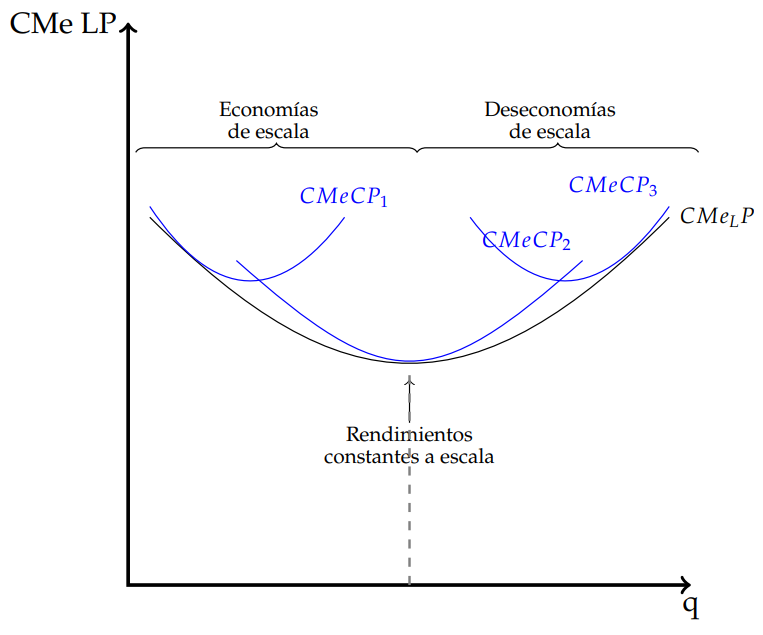
\includegraphics[scale=0.6]{../Figures/C13.10.png}
\end{frame}

\begin{frame}
    \frametitle{Rendimientos a escala}
    Esto se resume en el siguiente cociente:
    \[ \frac{\Delta \% Q}{\Delta \% I} \]
    \begin{itemize}
        \item Si el cociente es mayor a 1, entonces hay rendimientos crecientes a escala
        \item Si el cociente es igual a 1, entonces hay rendimientos constantes a escala
        \item Si el cociente es menor a 1, entonces hay rendimientos decrecientes a escala
    \end{itemize}
\end{frame}

\begin{frame}{Ejemplo - Economías de escala}
    \begin{itemize}
    \item Las industrias químicas utilizan una gran cantidad de tuberías para transportar su producción. 
    \item ¿Cuánto cuesta construir la tubería? Depende de la circunferencia (la pared de la tubería es una hoja de metal enrollada)
    \item Pero la cantidad de producto que puede pasar por la tubería está determinado por el área
    \end{itemize}

    \begin{table}[h]
    \centering
    \renewcommand{\arraystretch}{1} % Espaciado entre filas
    \begin{adjustbox}{width=0.8\textwidth}
    \begin{tabular}{lcc}
    \toprule
    \textbf{Tamaño de la tubería} & \textbf{Circunferencia (\(2\pi r\))} & \textbf{Área (\(\pi r^2\))} \\
    \midrule
    Pequeña ($d =4; r=2$) & 12.5 pulgadas  & 12.5 pulgadas²  \\
    Mediana ($d =8; r=4$) & 25.1 pulgadas  & 50.2 pulgadas²  \\
    Grande ($d =16; r=8$) & 50.2 pulgadas  & 201.1 pulgadas² \\
    \bottomrule
    \end{tabular}
    \end{adjustbox}
    \end{table}
    \centering
    \begin{itemize}
    \item Una duplicación del costo de producción de la tubería (diámetro) permite que la empresa química produzca cuatro veces más material. 
    \[ \frac{\Delta \% Q}{\Delta \% I} =\frac{ 300\% }{100\%}=3\]
    \end{itemize}
\end{frame}

\begin{frame}{Ejemplo - Deseconomías de escala}
    \begin{itemize}
        \item Una empresa de consultoría crece significativamente contratando más empleados para aumentar su capacidad de atención.
        \item Al aumentar significativamente la cantidad de empleados, los costos administrativos (supervisión, coordinación y comunicación interna) crecen desproporcionadamente.
        \item Esto genera deseconomías de escala: el aumento proporcional de los insumos lleva a un aumento menos que proporcional del producto.
    \end{itemize}

    \begin{table}[h]
    \centering
    \renewcommand{\arraystretch}{1} % Espaciado entre filas
    \begin{adjustbox}{width=0.8\textwidth}
    \begin{tabular}{lccc}
    \toprule
    \textbf{Escala} & \textbf{Salarios} & \textbf{Horas efectivas totales} & \textbf{CMeT} \\
    \midrule
    Pequeña (10 empleados)  & \$5000 mensuales  & 1.600 horas & \$3.125 \\
    Mediana (20 empleados)  & \$10000 mensuales  & 2.800 horas & $\sim$ \$3.6 \\
    Grande (40 empleados)   & \$20000 mensuales  & 4.200 horas & $\sim$ \$4.75 \\
    \bottomrule
    \end{tabular}
    \end{adjustbox}
    \end{table}

    \centering
    \begin{itemize}
        \item Al duplicar los insumos (cantidad de empleados), la producción total aumenta en menor proporción (solo un 75\%), indicando claramente deseconomías de escala.
    \end{itemize}

    \[
    \frac{\Delta \% Q}{\Delta \% I} = \frac{75\%}{100\%} = 0.75
    \]
\end{frame}

\begin{frame}{¿Por qué aumentar costos medios puede convenir?}
    \begin{itemize}
        \item Aunque al aumentar la cantidad de empleados la empresa incrementa sus costos medios, podría ser racional hacerlo si el ingreso adicional por la mayor producción supera el incremento en los costos.
        \item Por ejemplo, supongamos que cada hora de consultoría se factura a \$10:
        \begin{itemize}
            \item Escala mediana: 2.800 horas $\times$ \$10 = \$28.000 mensuales.
            \item Escala grande: 4.200 horas $\times$ \$10 = \$42.000 mensuales.
        \end{itemize}
        \item Aunque el beneficio por hora disminuye ($\$10-\$4.75$ en lugar de $\$10-\$3.6$), el beneficio total aumenta.
        \begin{itemize}
            \item Escala mediana: \$28.000 - \$10.000 = \$18.000.
            \item Escala grande: \$42.000 - \$20.000 = \$22.000.
        \end{itemize}
    \end{itemize}
    \begin{boxA}
        \small Incrementar costos medios es racional siempre que el ingreso adicional supere al aumento de costos.
    \end{boxA}
\end{frame}


\begin{frame}{Costos de Largo Plazo en la práctica}

    \begin{figure}[ht]
        \centering
        \begin{tikzpicture}
        
        % Ejes
        \draw[thick,->] (0,0) -- (6,0) node[right] {$q$};
        \draw[thick,->] (0,0) -- (0,5) node[above] {Costos};
        
        % Curva CMeLP con tramo constante
        \draw[thick, domain=0.75:3, smooth, variable=\x] plot ({\x}, {3/(\x)+0.5});
        \draw[thick] (3,1.5) -- (5.5,1.5);
        
        % Etiqueta de curva
        \node[right] at (5.5,1.5) {$CMe_{LP}$};
        
        % Punto mínimo
        \draw[dashed] (3,0) node[below] {$q_{min}$} -- (3,1.5);
        \filldraw (3,1.5) circle (2pt);
        
        \end{tikzpicture}
        \caption{Curva de costos medios de largo plazo con tramo constante.}
        \end{figure}
\end{frame}

\begin{frame}{Costos de Largo Plazo en la práctica}
    \begin{figure}[h!]
        \centering
        \begin{tikzpicture}[scale=1]
        % Ejes
        \draw[thick,->] (0,0) -- (6,0) node[right] {$q$};
        \draw[thick,->] (0,0) -- (0,5) node[above] {Costos};
        
        % Curva CMeLP
        \draw[thick, domain=0.3:5.5, smooth, variable=\x] plot ({\x}, {1/\x+1});
        
        % Etiqueta curva
        \node[right] at (5.5,1.18) {\textit{CMe}$_{LP}$};
        
        \end{tikzpicture}
        \caption{Curva de costos medios de largo plazo para monopolios naturales.}
        \end{figure}
\end{frame}

\begin{frame}
    \frametitle{La oferta del mercado}
    \begin{boxA}
        \centering
        La oferta del mercado refleja la cantidad de bienes que se va ofertar de manera conjunta en el mercado a cada precio. Por lo tanto, se obtiene mediante la suma de las cantidades de bienes que ofrece cada uno los productores a cada precio.
    \end{boxA}
    \renewcommand{\arraystretch}{1.2} % Espaciado entre filas
    \begin{table}[h]
        \centering
        \rowcolors{2}{gray!10}{white} % Alternar colores en las filas
        \setlength{\arrayrulewidth}{1pt} % Grosor de líneas
        \arrayrulecolor{black} % Color de líneas
        \begin{tabular}{|c|c|c|c|c|}
            \hline
            \rowcolor{blue!20} % Color de la primera fila (encabezado)
            \textbf{P} & \textbf{QEmpresa$_1$} & \textbf{QEmpresa$_2$} & \textbf{QEmpresa$_3$} & \textbf{QTotal} \\
            \hline
            0  & 4  & 0  & 0  & 4  \\
            10 & 6  & 0  & 10 & 16 \\
            20 & 8  & 0  & 20 & 28 \\
            30 & 10 & 0  & 30 & 40 \\
            40 & 12 & 20 & 40 & 72 \\
            50 & 14 & 30 & 50 & 94 \\
            60 & 16 & 40 & 60 & 116 \\
            \hline
        \end{tabular}
    \end{table}
\end{frame}

\begin{frame}{La oferta del mercado}
    \centering
    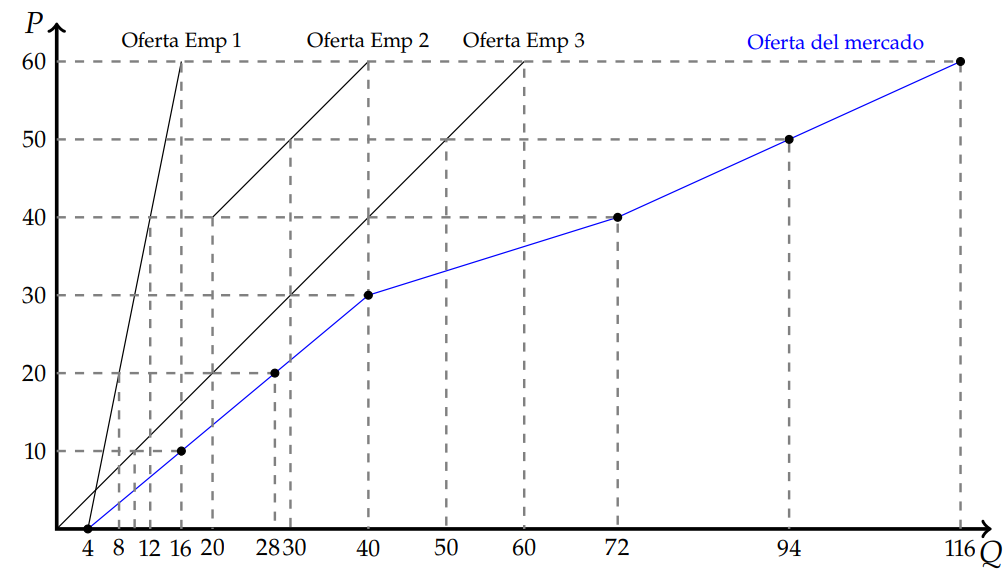
\includegraphics[scale=0.5]{../Figures/C14.1.png}
\end{frame}

\begin{frame}{La interpretación de la oferta del mercado}
    \begin{itemize}
        \item La oferta del mercado refleja la cantidad de bienes que se va ofrecer de manera conjunta en el mercado a cada precio.
        \item Alternativamente, se puede interpretar como la mínima disposición a cobrar que tienen los productores para cada cantidad del producto que venden.
    \end{itemize}
    \begin{center}
        \begin{tikzpicture}[scale=0.65]
        \draw[thick,->] (0,0) -- (8,0) node[below] {$Q$};
        \draw[thick,->] (0,0) -- (0,6.5) node[left] {$P$};
        \draw [thick] (1,2) -- (7,5);
        \node [right] at (7.1,5.2) {Oferta};
        % Punto A
        \node [right] at (3,3.6) {$A$};
        \fill (3.2,3.1) circle (3pt);
        \draw[dashed, gray] (3.2,0) -- (3.2,3.1);
        \draw[dashed, gray] (0,3.1) -- (3.2,3.1);
        \node[below] at (3.2,0) {40};
        \node[left] at (0,3.1) {30};
        \end{tikzpicture}
    \end{center}
\end{frame}

\begin{frame}{Desplazamientos \textbf{sobre} la curva de oferta}
        \begin{itemize}
            \item Si cambia el \textbf{precio} del producto, se modifica su \textbf{cantidad ofrecida}.
            \item La curva de oferta no se modifica, nos desplazamos \textbf{sobre} la curva.\vspace{1mm}
        \end{itemize}
        \begin{center}
            \begin{tikzpicture}[scale=0.8]
            \draw[thick,->] (0,0) -- (8,0) node[below] {$Q$};
            \draw[thick,->] (0,0) -- (0,6.5) node[left] {$P$};
            \draw [thick] (1,2) -- (7,5);
            \node [right] at (7.1,5.2) {Oferta};
            % Punto A
            \node [right] at (3.1,3.5) {$A$};
            \fill (3.2,3.1) circle (3pt);
            \draw[dashed, gray] (3.2,0) -- (3.2,3.1);
            \draw[dashed, gray] (0,3.1) -- (3.2,3.1);
            \node[below] at (3.2,0) {40};
            \node[left] at (0,3.1) {30};
            % Punto B
            \node [right] at (5.5,4.7) {$B$};
            \fill (5.6,4.3) circle (3pt);
            \draw[dashed, gray] (5.6,0) -- (5.6,4.3);
            \draw[dashed, gray] (0,4.3) -- (5.6,4.3);
            \node[below] at (5.6,0) {60};
            \node[left] at (0,4.3) {40};
            \end{tikzpicture}
        \end{center}
    \end{frame}

\begin{frame}{Factores que afectan a la curva de oferta}
    \begin{itemize}
        \item La tecnología y sus cambio
        \item El precio de los insumos requeridos para la producción
        \item El número de vendedores que puede variar en el mercado
        \item Las distintas políticas gubernamentales (como por ejemplo los impuestos)
        \item Las expectativas de los productores
        \item Otras influencias externas (como por ejemplo el clima en el caso de productos agrícolas)  
    \end{itemize}
    \begin{boxB}
        \begin{center}
          No confundir cambios en la oferta con cambios \\ en las cantidades ofrecidas
        \end{center}
    \end{boxB}
\end{frame}

\begin{frame}
\frametitle{Algunos ejemplos}
    \begin{center}
    
\includegraphics[scale=0.35]{../Figures/M6.1.png}
    \end{center}
\end{frame}

\begin{frame}
\frametitle{Algunos ejemplos}
    \begin{center}
    
\includegraphics[scale=0.35]{../Figures/M6.2.png}
    \end{center}
\end{frame}

\begin{frame}
\frametitle{Algunos ejemplos}
    \begin{center}
    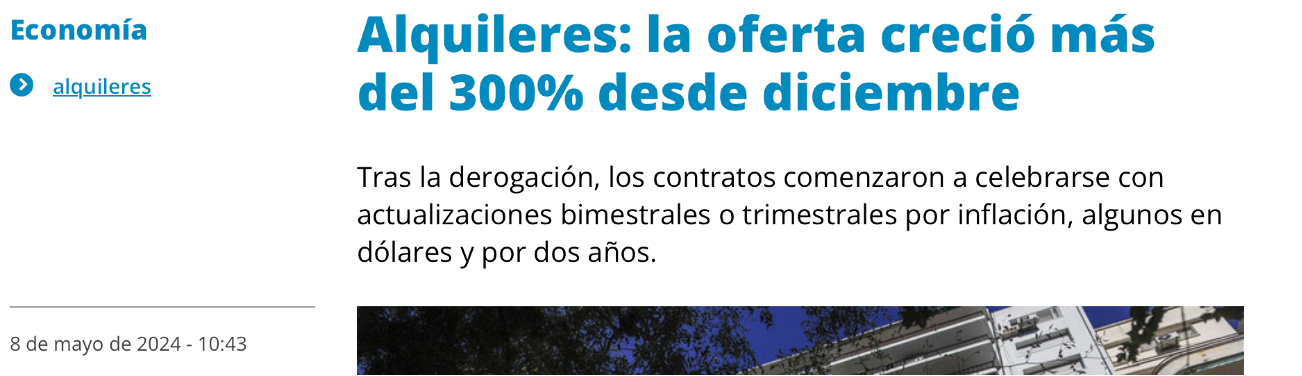
\includegraphics[scale=0.5]{../Figures/M6.3.png}
    \end{center}
\end{frame}

\begin{frame}
\frametitle{Algunos ejemplos}
    \begin{center}
    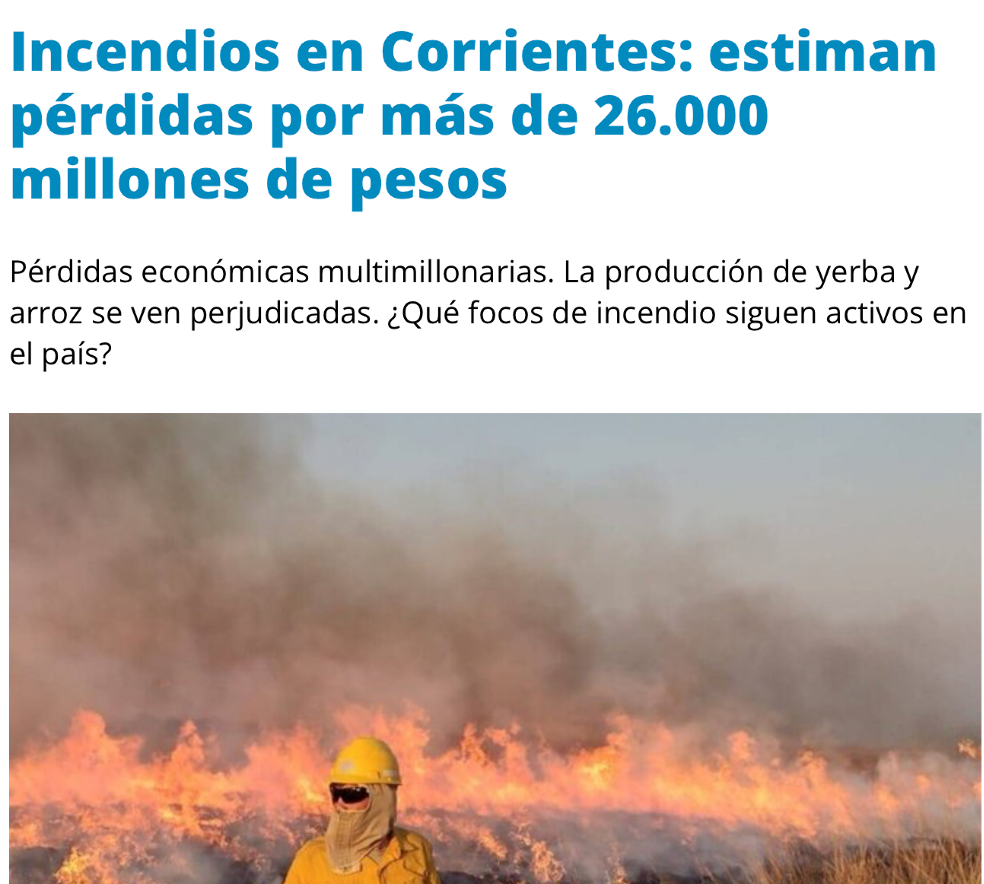
\includegraphics[scale=0.45]{../Figures/M6.4.png}
    \end{center}
\end{frame}

\end{document}